\subsection{Cameras}
After obtaining two of the MT9V034 cameras chosen through the process referenced in Appendix item \ref{camdecision}, several steps were taken to obtain test data from each camera. These steps are outlined in the following sections.

\subsubsection{Camera Breakout Boards}
\begin{figure}[H]
	\centerline{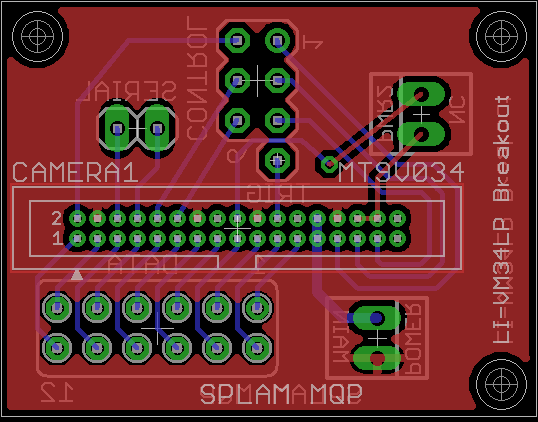
\includegraphics[width=0.5\textwidth]{camera_board.png}}
	\caption{LI-VM34LP Breakout Board}
	\label{camBreakoutBoard}
\end{figure}

\subsubsection{I$^2$C Control} 
Started by trying to get the camera version...
\begin{figure}[H]
	\centerline{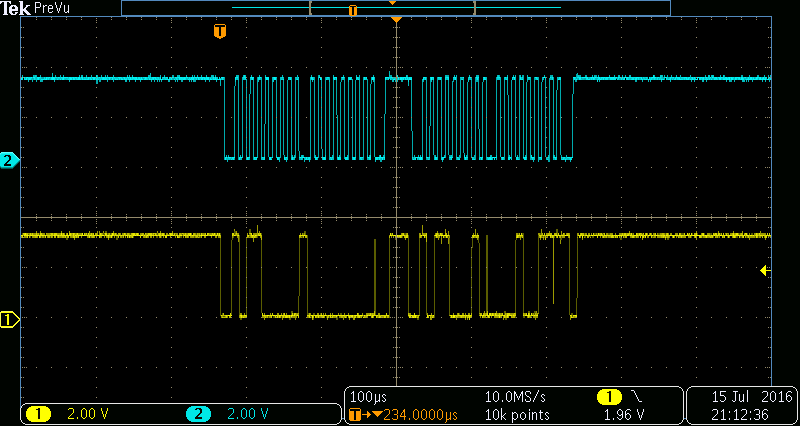
\includegraphics[width=1.0\textwidth]{oScope/i2c_0x00/tek00001.png}}
	\caption{Example I$^2$C Transfer with Camera}
	\label{camVersion}
\end{figure}

\par
Next, set camera control register for trigger mode and confirmed that it was working


\subsubsection{Camera Output}

Normal mode of operation.....
\begin{figure}[H]
	\centerline{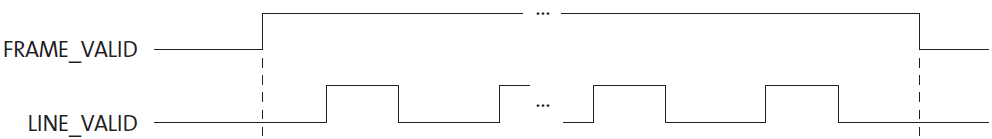
\includegraphics[width=1.0\textwidth]{camFvLv.png}}
	\caption{Frame and Line Valid}
	\label{FvLv}
\end{figure}
\begin{figure}[H]
	\centerline{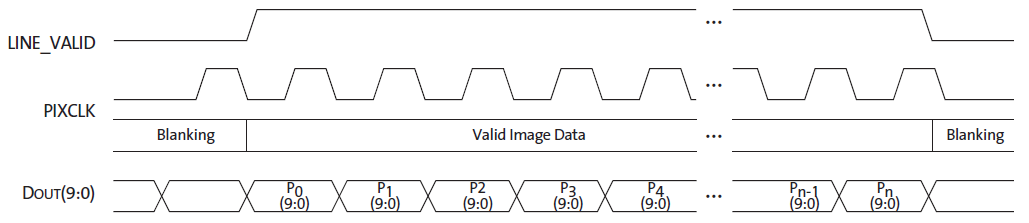
\includegraphics[width=1.0\textwidth]{camLvPckDout.png}}
	\caption{Line Data Transfer}
	\label{LvDout}
\end{figure}

\par
Grabbing an image of normal ops...
\begin{figure}[H]
	\centerline{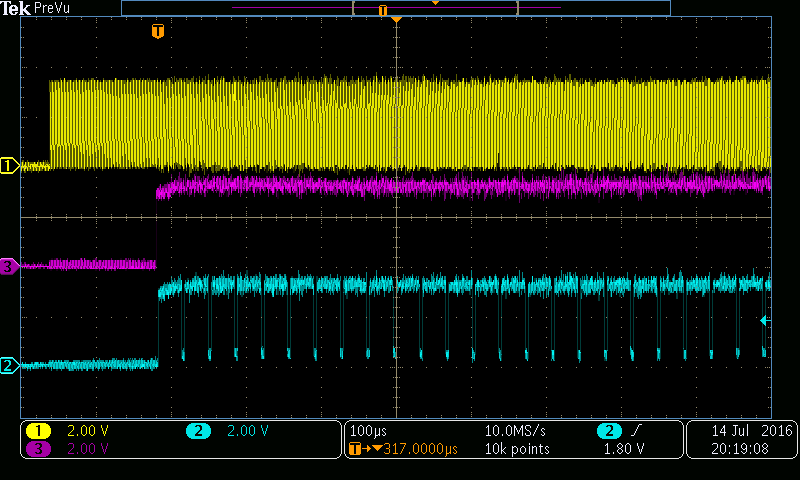
\includegraphics[width=1.0\textwidth]{oScope/pclk_fv_lv/tek00003.png}}
	\caption{Camera Data Transfer}
	\label{camDataTransfer}
\end{figure}

\par
triggered!

\begin{figure}[H]
	\centerline{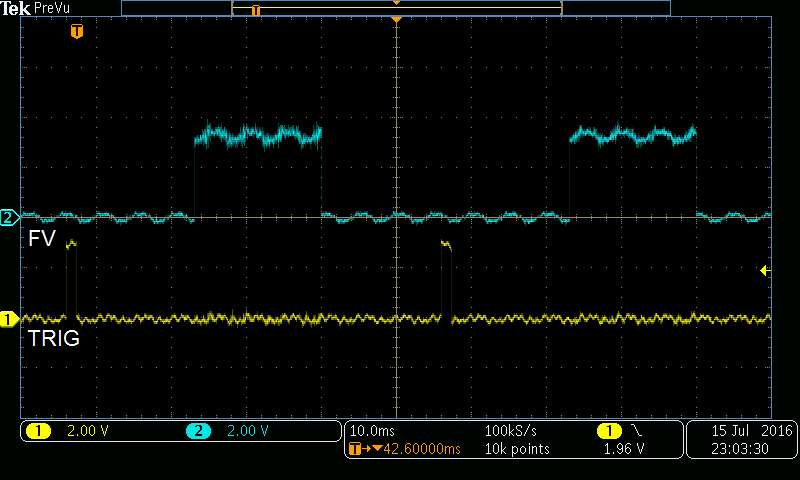
\includegraphics[width=1.0\textwidth]{oScope/i2c_0x07/externalTrigger/externalTrig.png}}
	\caption{Camera Running in Trigger Mode}
	\label{camInTrigMode}
\end{figure}


\subsubsection{Data Management}
AL422B FIFO, etc...

\begin{figure}[H]
	\centerline{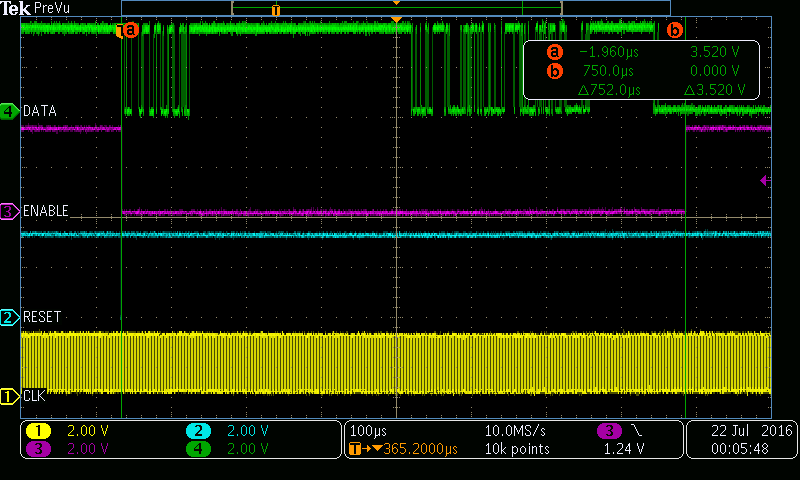
\includegraphics[width=1.0\textwidth]{oScope/camera_fifo/fifo_rstAndDataTimed.png}}
	\caption{Transferring Line Data from FIFO to FPGA}
	\label{fifoDataOut}
\end{figure}

\subsubsection{Transmitting Images Over UART for Analysis}
throw in screenshot of PuTTy
\begin{figure}[H]
	\centerline{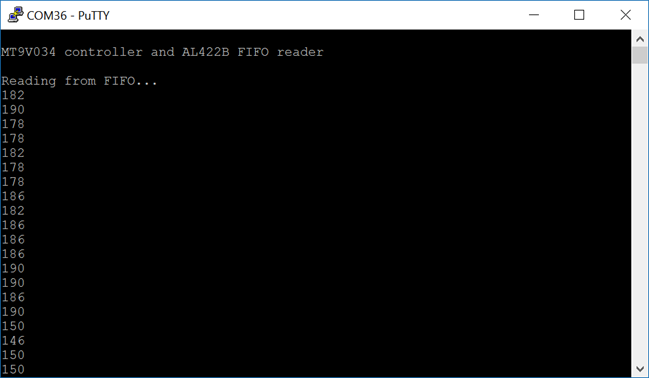
\includegraphics[width=0.6\textwidth]{oScope/camera_fifo/PuTTy.png}}
	\caption{Reading FIFO Data}
	\label{PuTTYfifoData}
\end{figure}

\par
After the image was recieved through PuTTy, the \textsc{Matlab} script found in Appendix item \ref{camTestMatlab} was used to parse the corresponding logfile into a greyscale image.
\begin{figure}[H]
	\centerline{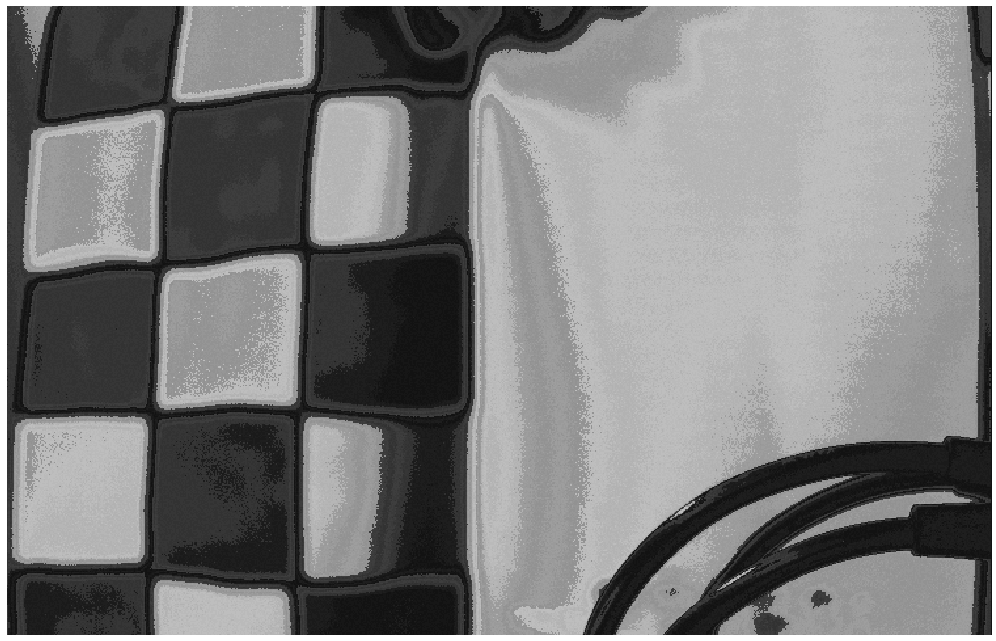
\includegraphics[width=0.75\textwidth]{oScope/camera_fifo/notebook.png}}
	\caption{Notebook With Grid and Oscilloscope Leads}
	\label{notebookImage}
\end{figure}